\chapter{The Photo-Electric Effect}
The photoelectric effect was the first direct experiment to demonstrate the quantum nature of electromagnetic energy transfer to and from matter. The purpose of this experiment is to verify Einstein's theory of the photoelectric effect, to measure Planck's constant, and to determine the work function for a surface.

\section{Physical Principles}
The photoelectric effect may be understood as a consequence of quantum mechanics, according to which light is carried by discrete bundles of energy (quanta) called photons.
Photons have energy $hf$, where $h$ is a universal constant called Planck's constant and $f$ is the frequency of the classical electromagnetic wave. When a photon is incident on a metallic surface, it interacts with an atom in the metal and transfers all its energy to one of the atom's electrons. This electron may then escape through the electric field at the surface, which keeps less energetic electrons inside the metal. The emerging electron then has energy equal to the energy of the photon minus the energy $W$ lost in escaping the metal. $W$, the \textbf{work function} of the surface, is a material-dependent constant. Since electrons also lose energy in collisions with other electrons before emerging, we may only specify the maximum possible energy for an electron liberated by light of frequency $f$ from a metal. If the material work function is $W$, this maximum energy\footnote{The maximum electron energy is measured in photoelectric experiments by finding the potential ($V$, in Volts) at which a decelerating electric field causes all electrons (charge $e$) to stop before reaching the electrode. Therefore, $E_{\mathrm{max}}=eV$.} is
\begin{equation}
  E_{\mathrm{max}}=hf-W
  \label{eq:emax}
\end{equation}

According to quantum mechanics, a plot of $E_{\mathrm{max}}$ against $f$ should give a straight line with slope $h$, as shown in the figure {\ref{fig:threshold}}. The line should intercept the $f$-axis at $f_0 = W / h$ . This value $f_0$, the lowest frequency that can eject an electron, is called the \textbf{threshold frequency}.
\begin{figure}[h]
\centering
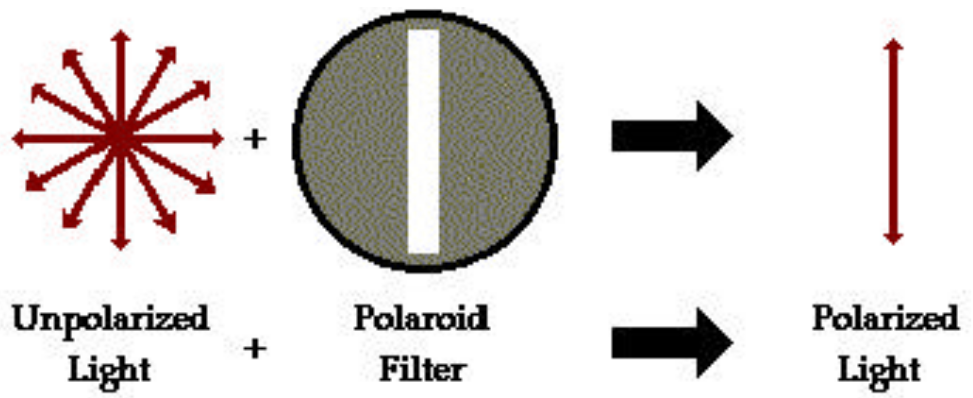
\includegraphics[width=0.8\textwidth]{./Exp8/pic/image1.png}
\caption{Maximum kinetic energy of the ejected electrons as a function of the frequency of the incident electromagnetic radiation}
\label{fig:threshold}
\end{figure} 

\section{Historical Perspective}
Early attempts to describe the photoelectric effect used classical electromagnetism. These studies concluded that the stopping voltage, or potential needed to keep the highest energy electrons from reaching the electrode, should depend only on the intensity of the light but not on the frequency. (In other words, the electrons should be ejected with more kinetic energy if you shine a bright light rather than a dim light.) But it turns out that experimental evidence contradicts these predictions! If you shine a light with any frequency below $f_0$, no electrons will be set free no matter how intense the light.\myskip

Albert Einstein was the first (in 1905) to analyze the photo-effect problem based on a concept of light as quantized energy packages. The idea earned him his Physics Nobel-Prize in 1921. The idea, though simple, was revolutionary at the time. Einstein hypothesized that light consists of little discreet energy packages, or quanta, which behave like particles called photons. An individual photon cannot be divided, but it can be totally absorbed under appropriate circumstances. The size of the photon energy quantum is just determined by the frequency $f$ of the electromagnetic light, as $E_{\mathrm{photon}}=hf$. For the electron that absorbs a photon to leave the metal requires a minimum energy $W$ to set it free. (The value of $W$ depends on the metal.) So after the electron leaves the metal, it still has energy $hf - W$, which it carries as kinetic energy. This is where equation ({\ref{eq:emax}}) comes from. \myskip

Does this mean that the all the classical electromagnetism you learned so far this semester is wrong? No! Electromagnetism is still a good theory that makes quantitative and correct predictions about the real world, so long as you deal with many photons and many atoms (i.e. in the macroscopic world). Only when it comes to the behavior of a single or few atoms, photons and/or electrons does one need to use Quantum Mechanics.\footnote{We said that classical electromagnetism claims that higher intensity means more energy in the light. This is still true. But classically, more intensity just means more photons, not photons of higher energy.}

\section{Experimental Apparatus}
The photoelectric effect in this experiment occurs at the cathode of an IP39 phototube. The phototube is constructed as shown in Figure {\ref{fig:phototube}}. The IP39 phototube is designed to function as a diode where light, incident on the tube, illuminates the cathode and causes photo-emission of electrons. The central wire (anode) is shielded from illumination.
\begin{figure}[h]
\centering
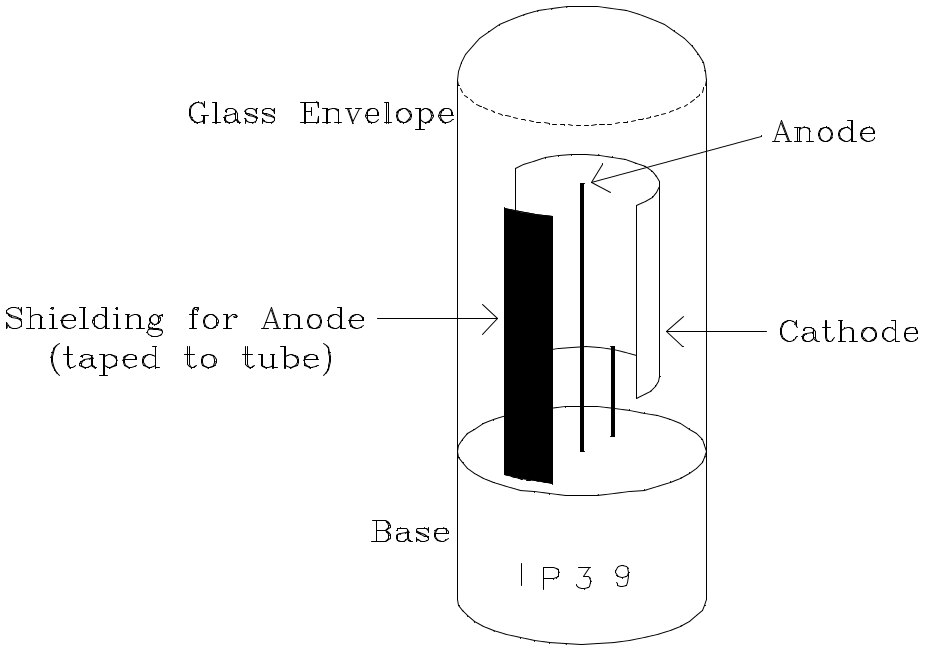
\includegraphics[width=0.5\textwidth]{./Exp8/pic/image2.png}
\caption{The IP39 Phototube}
\label{fig:phototube}
\end{figure} 

If the anode is connected through an external circuit to the cathode, a current will flow whenever the cathode is illuminated with light of frequency greater than $f_0$. If a potential $V$ is applied so that the anode is \emph{negative} with respect to the cathode, as illustrated in Figure {\ref{fig:scircuit}}, the emitted electrons will lose kinetic energy as they travel through the potential field. Electrons with kinetic energy less than $eV$ will not be able to reach the anode, and the current in the external circuit will be less than it would if $V = 0$. For a potential $V = V_S = E_{\mathrm{max}} / e$ , called the \textbf{stopping potential}, the current will drop to zero.
\begin{figure}[h]
\centering
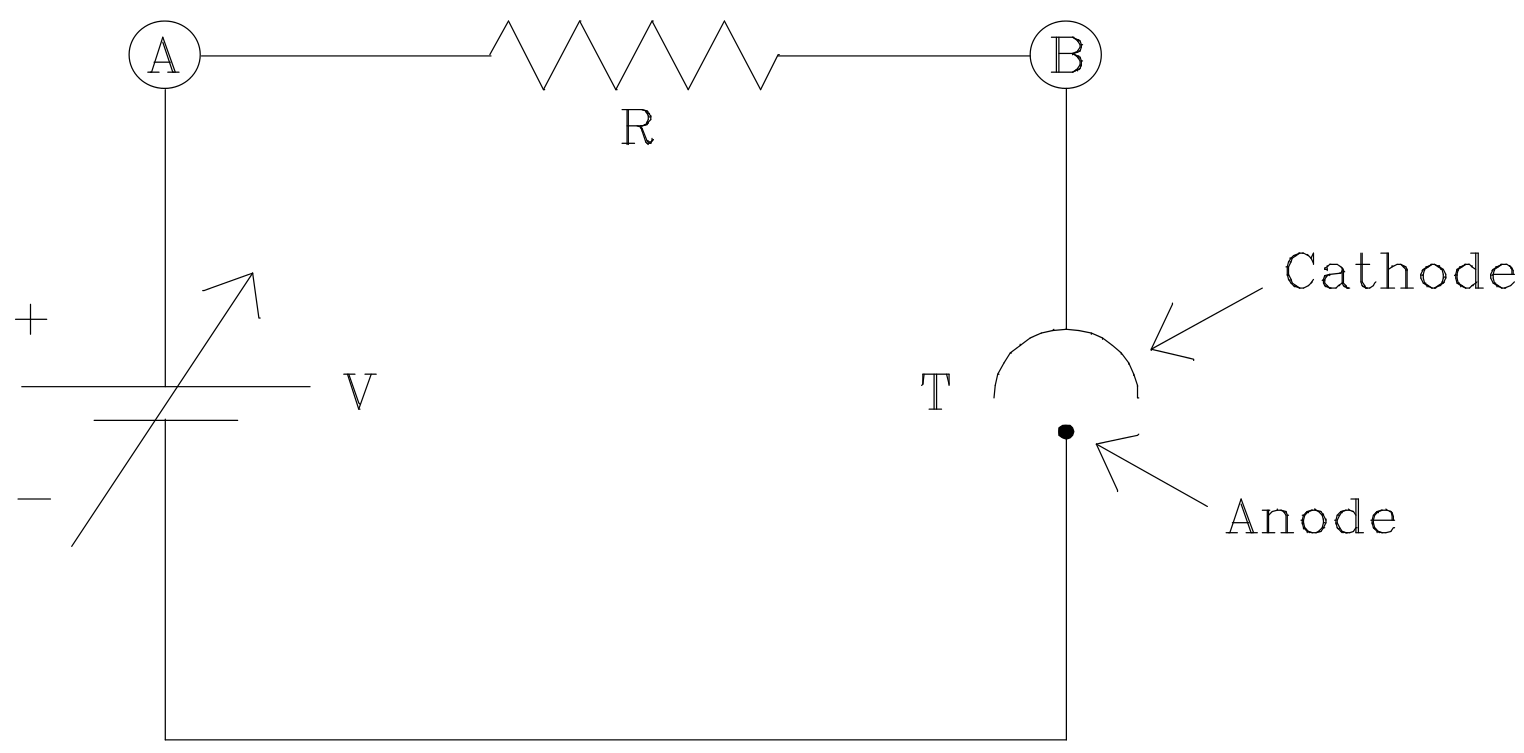
\includegraphics[width=0.5\textwidth]{./Exp8/pic/image3.png}
\caption{Simplified Phototube Circuit}
\label{fig:scircuit}
\end{figure} 

In more detail, as $V$ is varied, there are three possible cases to consider (see Figure {\ref{fig:scircuit}}):

\begin{description}
\item[Case I: $V < V_S$].  In this case, the anode (the symbol for the anode is the dot) will collect electrons. The tube $T$ will act like a battery of greater strength than $V$, and the electrons will flow around the circuit in a clockwise direction. The current will cause an $iR$ drop across $R$. Thus, $A$ and $B$ will be at different potentials.
\item[Case II: $V = V_S$].  At this critical value of $V$, electrons are just not energetic enough to reach the anode. No current flows, and $A$ and $B$ are at the same potential.
\item[Case III: $V > V_S$].  One might think that electrons would flow counterclockwise. This can happen if there is light striking the anode. If no light is permitted to strike the anode, no electrons are emitted from it and thus the tube $T$ acts like an open circuit; $A$ and $B$ are again at the same potential.
\end{description}

In principle, the stopping potential (for a given frequency of incident light) could be measured by finding with a voltmeter the value of the adjustable negative voltage $V$ at which the current passing through an ammeter in series with the phototube goes to zero. However, the number of photoelectrons liberated by available light sources produces currents of less than 2 microamperes, too small to be measured by simple meters. A more sensitive way is needed to determine the presence or absence of current in the phototube circuit. \myskip

A Photoelectric Module has been designed using high gain current amplifiers for easy measurement of the stopping potential for the IP39 phototube for several different frequencies of incident light. A schematic diagram of the phototube circuit using the Photo-electric Module is shown in Figure {\ref{fig:circuit}}. The High Gain Difference Amplifier is used to detect any current flowing through the resistor $R$ and consequently through the phototube. Both the High Gain Difference Amplifier and the $0$-$3\,\mathrm{V}$ meter are designed to draw negligible current from the phototube circuit. If the \textbf{Zero Adjust} control has been correctly set, then a reading of zero on the 5-0-5 meter means that no current is flowing through the phototube. The stopping potential applied to the phototube is set using the \textbf{Voltage Adjust} control and read with the $0$-$3\,\mathrm{V}$ meter.
\begin{figure}[h]
\centering
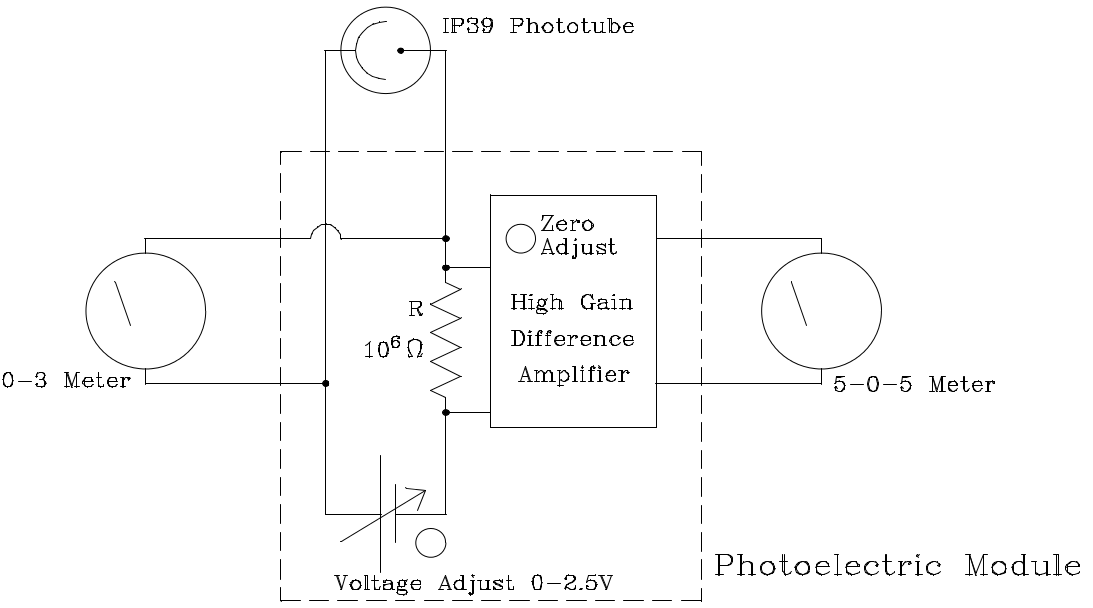
\includegraphics[width=0.8\textwidth]{./Exp8/pic/image4.png}
\caption{Schematic Diagram of the Phototube Circuit Using the Photo-electric Module}
\label{fig:circuit}
\end{figure} 

The overall arrangement of the apparatus is shown in Figure {\ref{fig:apparatus}} below. The Phototube circuitry is housed in the Photoelectric Module, which is connected externally to the two voltmeters as well as the Phototube. The Phototube itself is attached over a window in the housing of a mercury arc source, which provides light that is passed through selected filters and then strikes the cathode of the tube. 
\begin{figure}[h]
\centering
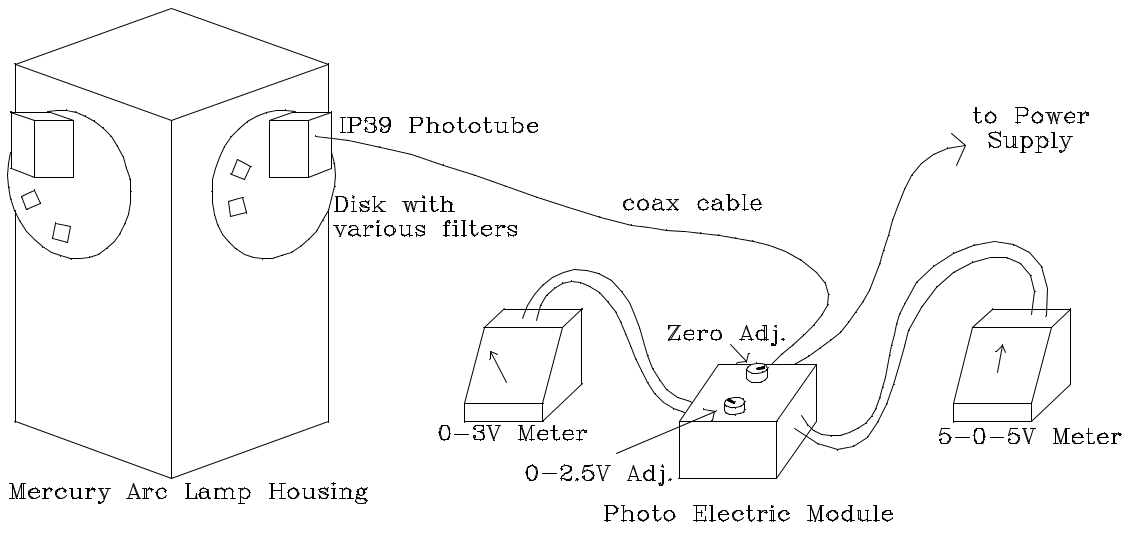
\includegraphics[width=0.8\textwidth]{./Exp8/pic/image5.png}
\caption{Arrangement of the Experimental Apparatus.}
\label{fig:apparatus}
\end{figure} 

In order to vary $f$, one would like to use an ideal \textbf{monochromator}, i.e., a source which produces light at a well-defined but variable frequency. A discharge tube, such as the mercury arc source, produces a series of discrete frequencies, i.e., \textbf{spectral lines}. A prism or grating spectrometer could be used to transmit any one of these lines while rejecting the others, but the narrow slits on such an instrument will not provide sufficient intensity for this experiment. Therefore, we use instead a set of bandpass optical filters, each of which transmits only a small band of frequencies. The arrangement is shown in Figure {\ref{fig:light}}.
\begin{figure}[h]
\centering
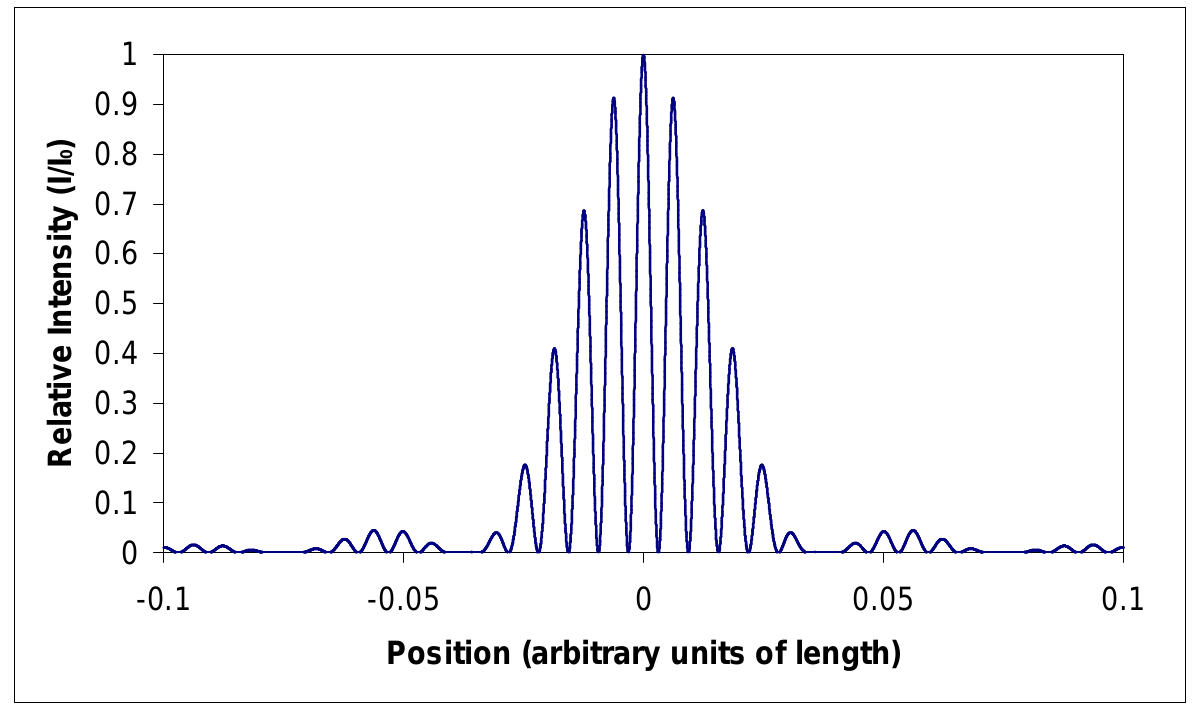
\includegraphics[width=0.8\textwidth]{./Exp8/pic/image6.png}
\caption{Light source and Phototube Arrangement.}
\label{fig:light}
\end{figure} 

Figure {\ref{fig:bandpass}} presents a graph indicating the percentage of light transmitted as a function of wavelength for the four filters to be used. On the same graph the principal wavelengths in the visible spectrum of mercury are indicated as straight lines.\myskip

 Although a filter may transmit more than one line, only the most energetic photons determine $E_{\mathrm{max}}$. (Note that the vertical scale of Figure {\ref{fig:bandpass}} is logarithmic; the \emph{small percentage} of the intensity of the most energetic lines passed by two of the filters is not sufficient to affect the results of this experiment.)

\begin{figure}[h]
\centering
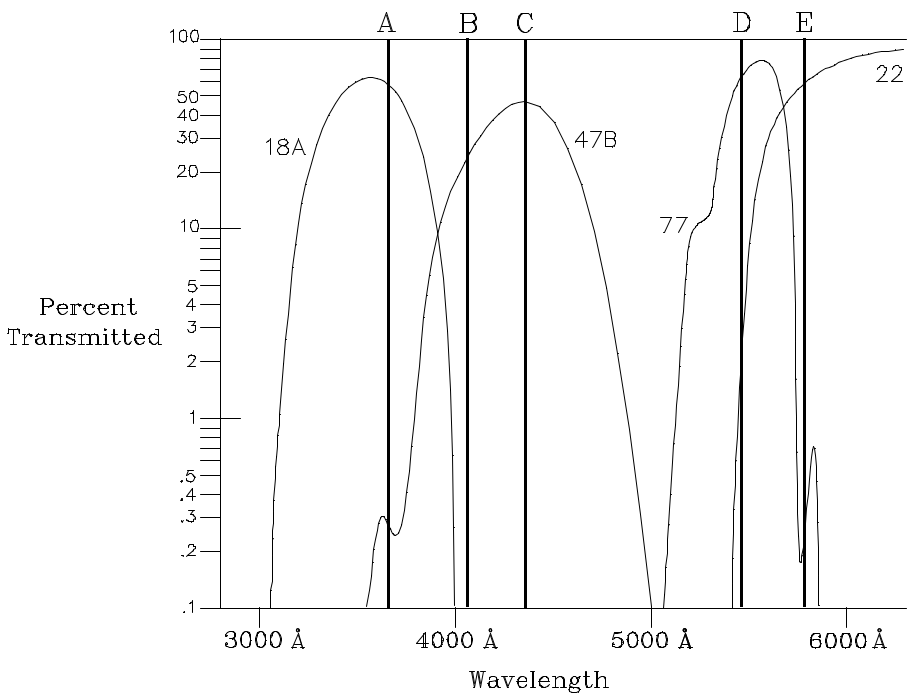
\includegraphics[width=0.8\textwidth]{./Exp8/pic/image7.png}
\caption{Percentage of Light Transmitted by Four Bandpass Filters.}
\label{fig:bandpass}
\end{figure} 

Mercury Lines Shown on Graph ($1\,\text{\AA} = 10^{-10}\, \mathrm{m}$)
\begin{table}[h]
  \centering
  \begin{tabular}{ll}
(A) Triplet: $3650\, \text{\AA}$, $3655\, \text{\AA}$, $3663\, \text{\AA}$&(D) Singlet: $5461\, \text{\AA}$\\
(B) Doublet: $4047\, \text{\AA}$, $4078\, \text{\AA}$&(E) Doublet: $5770\, \text{\AA}$, $5791\, \text{\AA}$\\
(C) Singlet: $4358\, \text{\AA}$&    
  \end{tabular}
\end{table}

\section{Procedure}
\subsection{Determining Planck's Constant $h$ and the Work Function $W$ of the Phototube}
$E_{\mathrm{max}}$ can be measured for a few different frequencies of incident radiation using the mercury arc source and filters as described above. The stopping potential for each filter can be determined using the Phototube circuit shown in Figure {\ref{fig:circuit}}. Turn on the power supply for the Photoelectric Module and the mercury lamp. Since the High Gain Difference Amplifier drifts slowly with time or temperature, it is important to set the Zero Adjust control before you start to make measurements.\myskip

First, turn the \textbf{Voltage Adjust Control} to the fully counterclockwise position. (The 0-3 meter should read 0.) Then, the \textbf{Zero Adjust} is set so that the 5-0-5 meter reads zero when no light is allowed to shine on the cathode. (The phototube is blocked by turning the filter disk to a no-window position. Note that the window which allows you to see light through the filter \emph{is \underline{not} the same as the window which allows light into the phototube housing}.) The Zero Adjust setting should be checked periodically. \myskip

Now, stopping potential measurements can be made. Rotate one of the filters into position between the light source and the phototube. The 5-0-5 meter should show a large deflection. Turn the Voltage Adjust knob clockwise until the reading on the 5-0-5 meter reads zero or near zero. Once the needle on the 5-0-5 meter stops moving toward zero, the stopping potential can be read from the 0-3 meter. Note: It is very important to carefully monitor the 5-0-5 meter when turning up the voltage across the phototube. \emph{The stopping potential is the \underline{minimum} voltage that stops the current flow through the phototube}. The stopping potential can be measured for other light frequencies by turning the Voltage Adjust to zero, selecting another filter, and repeating the above procedure. Plot $V_{S}$ versus $f$ and determine $h$ and $W$.

\subsection{Disproving the Classical Theory}
The classical theory (Newtonian mechanics and classical electromagnetism) predicts that if the \emph{intensity} of the light is cut in half, then the stopping potential will likewise be cut in half. Use the filter which is half masked with aluminum foil and see whether the stopping potential remains the same as with the equivalent unmasked filter. \myskip

\underline{Questions:}
\begin{enumerate}
\item Why is the anode of the phototube shielded from light?

\item If the light on the phototube contains two different wavelengths $\lambda_{1}$ and $\lambda_{2}$, which value must be used in the formula for the stopping potential? What is the effect of light of the other wavelength?

\item Does your value for the work function $W$ of the tube have the order of magnitude you expected? Why did you expect (or not expect) the work function to be of this magnitude?

\item What are the experimental features of the photoelectric effect that Newtonian mechanics and classical electromagnetic theory cannot explain? 

\item The surface of the photocathode of the IP39 tube is an alloy of cesium and antimony. Impurities (atoms from the anode, for example) can sometimes become deposited on the cathode surface. What effect would such a deposit have? How would it affect your values for the stopping voltages? Decide from your data whether this effect may be important for your tube.
\end{enumerate}
